\documentclass[]{article}
\usepackage{lmodern}
\usepackage{amssymb,amsmath}
\usepackage{ifxetex,ifluatex}
\usepackage{fixltx2e} % provides \textsubscript
\ifnum 0\ifxetex 1\fi\ifluatex 1\fi=0 % if pdftex
  \usepackage[T1]{fontenc}
  \usepackage[utf8]{inputenc}
\else % if luatex or xelatex
  \ifxetex
    \usepackage{mathspec}
  \else
    \usepackage{fontspec}
  \fi
  \defaultfontfeatures{Ligatures=TeX,Scale=MatchLowercase}
\fi
% use upquote if available, for straight quotes in verbatim environments
\IfFileExists{upquote.sty}{\usepackage{upquote}}{}
% use microtype if available
\IfFileExists{microtype.sty}{%
\usepackage{microtype}
\UseMicrotypeSet[protrusion]{basicmath} % disable protrusion for tt fonts
}{}
\usepackage[margin=1in]{geometry}
\usepackage{hyperref}
\hypersetup{unicode=true,
            pdfborder={0 0 0},
            breaklinks=true}
\urlstyle{same}  % don't use monospace font for urls
\usepackage{longtable,booktabs}
\usepackage{graphicx,grffile}
\makeatletter
\def\maxwidth{\ifdim\Gin@nat@width>\linewidth\linewidth\else\Gin@nat@width\fi}
\def\maxheight{\ifdim\Gin@nat@height>\textheight\textheight\else\Gin@nat@height\fi}
\makeatother
% Scale images if necessary, so that they will not overflow the page
% margins by default, and it is still possible to overwrite the defaults
% using explicit options in \includegraphics[width, height, ...]{}
\setkeys{Gin}{width=\maxwidth,height=\maxheight,keepaspectratio}
\IfFileExists{parskip.sty}{%
\usepackage{parskip}
}{% else
\setlength{\parindent}{0pt}
\setlength{\parskip}{6pt plus 2pt minus 1pt}
}
\setlength{\emergencystretch}{3em}  % prevent overfull lines
\providecommand{\tightlist}{%
  \setlength{\itemsep}{0pt}\setlength{\parskip}{0pt}}
\setcounter{secnumdepth}{0}
% Redefines (sub)paragraphs to behave more like sections
\ifx\paragraph\undefined\else
\let\oldparagraph\paragraph
\renewcommand{\paragraph}[1]{\oldparagraph{#1}\mbox{}}
\fi
\ifx\subparagraph\undefined\else
\let\oldsubparagraph\subparagraph
\renewcommand{\subparagraph}[1]{\oldsubparagraph{#1}\mbox{}}
\fi

%%% Use protect on footnotes to avoid problems with footnotes in titles
\let\rmarkdownfootnote\footnote%
\def\footnote{\protect\rmarkdownfootnote}

%%% Change title format to be more compact
\usepackage{titling}

% Create subtitle command for use in maketitle
\newcommand{\subtitle}[1]{
  \posttitle{
    \begin{center}\large#1\end{center}
    }
}

\setlength{\droptitle}{-2em}

  \title{}
    \pretitle{\vspace{\droptitle}}
  \posttitle{}
    \author{}
    \preauthor{}\postauthor{}
    \date{}
    \predate{}\postdate{}
  
\usepackage{booktabs}
\usepackage{longtable}
\usepackage{array}
\usepackage{multirow}
\usepackage[table]{xcolor}
\usepackage{wrapfig}
\usepackage{float}
\usepackage{colortbl}
\usepackage{pdflscape}
\usepackage{tabu}
\usepackage{threeparttable}
\usepackage{threeparttablex}
\usepackage[normalem]{ulem}
\usepackage{makecell}

\usepackage{leading}
\leading{18pt}

\begin{document}

--

\textbf{Table 1}

\begin{longtable}[]{@{}lll@{}}
\toprule
Family & Genus & Species\tabularnewline
\midrule
\endhead
Brassicaceae & Brassica & Brassica rapa\tabularnewline
Brassicaceae & Brassica & Brassica oleracea\tabularnewline
Brassicaceae & Eruca & Eruca versicaria\tabularnewline
Brassicaceae & Sinapis & Sinapis alba\tabularnewline
Convolvulaceae & Ipomoea & Ipomoea aquatica\tabularnewline
Convolvulaceae & Ipomoea & Ipomoea purpurea\tabularnewline
Solanaceae & Capsicum & Capsicum annuum\tabularnewline
Solanaceae & Petunia & Petunia integrifolia\tabularnewline
Solanaceae & Solanum & Solanum lycopersicum\tabularnewline
Solanaceae & Solanum & Solanum melongena\tabularnewline
\bottomrule
\end{longtable}

\newpage

\newpage

\textbf{Table 3}

\begin{longtable}[]{@{}lllr@{}}
\toprule
Family & Species & Donor & Seeds\tabularnewline
\midrule
\endhead
Brassicaceae & B. oleracea & C. annuum & 5\tabularnewline
Brassicaceae & B. rapa & B. oleracea & 2\tabularnewline
Brassicaceae & B. rapa & B. oleracea & 13\tabularnewline
Brassicaceae & B. rapa & S. lycopersicum & 1\tabularnewline
Brassicaceae & B. rapa & B. oleracea & 7\tabularnewline
Brassicaceae & B. rapa & B. oleracea & 5\tabularnewline
Brassicaceae & S. alba & B. oleracea & 7\tabularnewline
Brassicaceae & E. sativa & C. annuum & 6\tabularnewline
Brassicaceae & E. sativa & C. annuum & 1\tabularnewline
Solanaceae & S. lycopersicum & S. alba & 3\tabularnewline
Solanaceae & S. melongena & P. integrifolia & 36\tabularnewline
Solanaceae & C. annuum & S. alba & 127\tabularnewline
Solanaceae & C. annuum & E. sativa & 3\tabularnewline
\bottomrule
\end{longtable}

\newpage

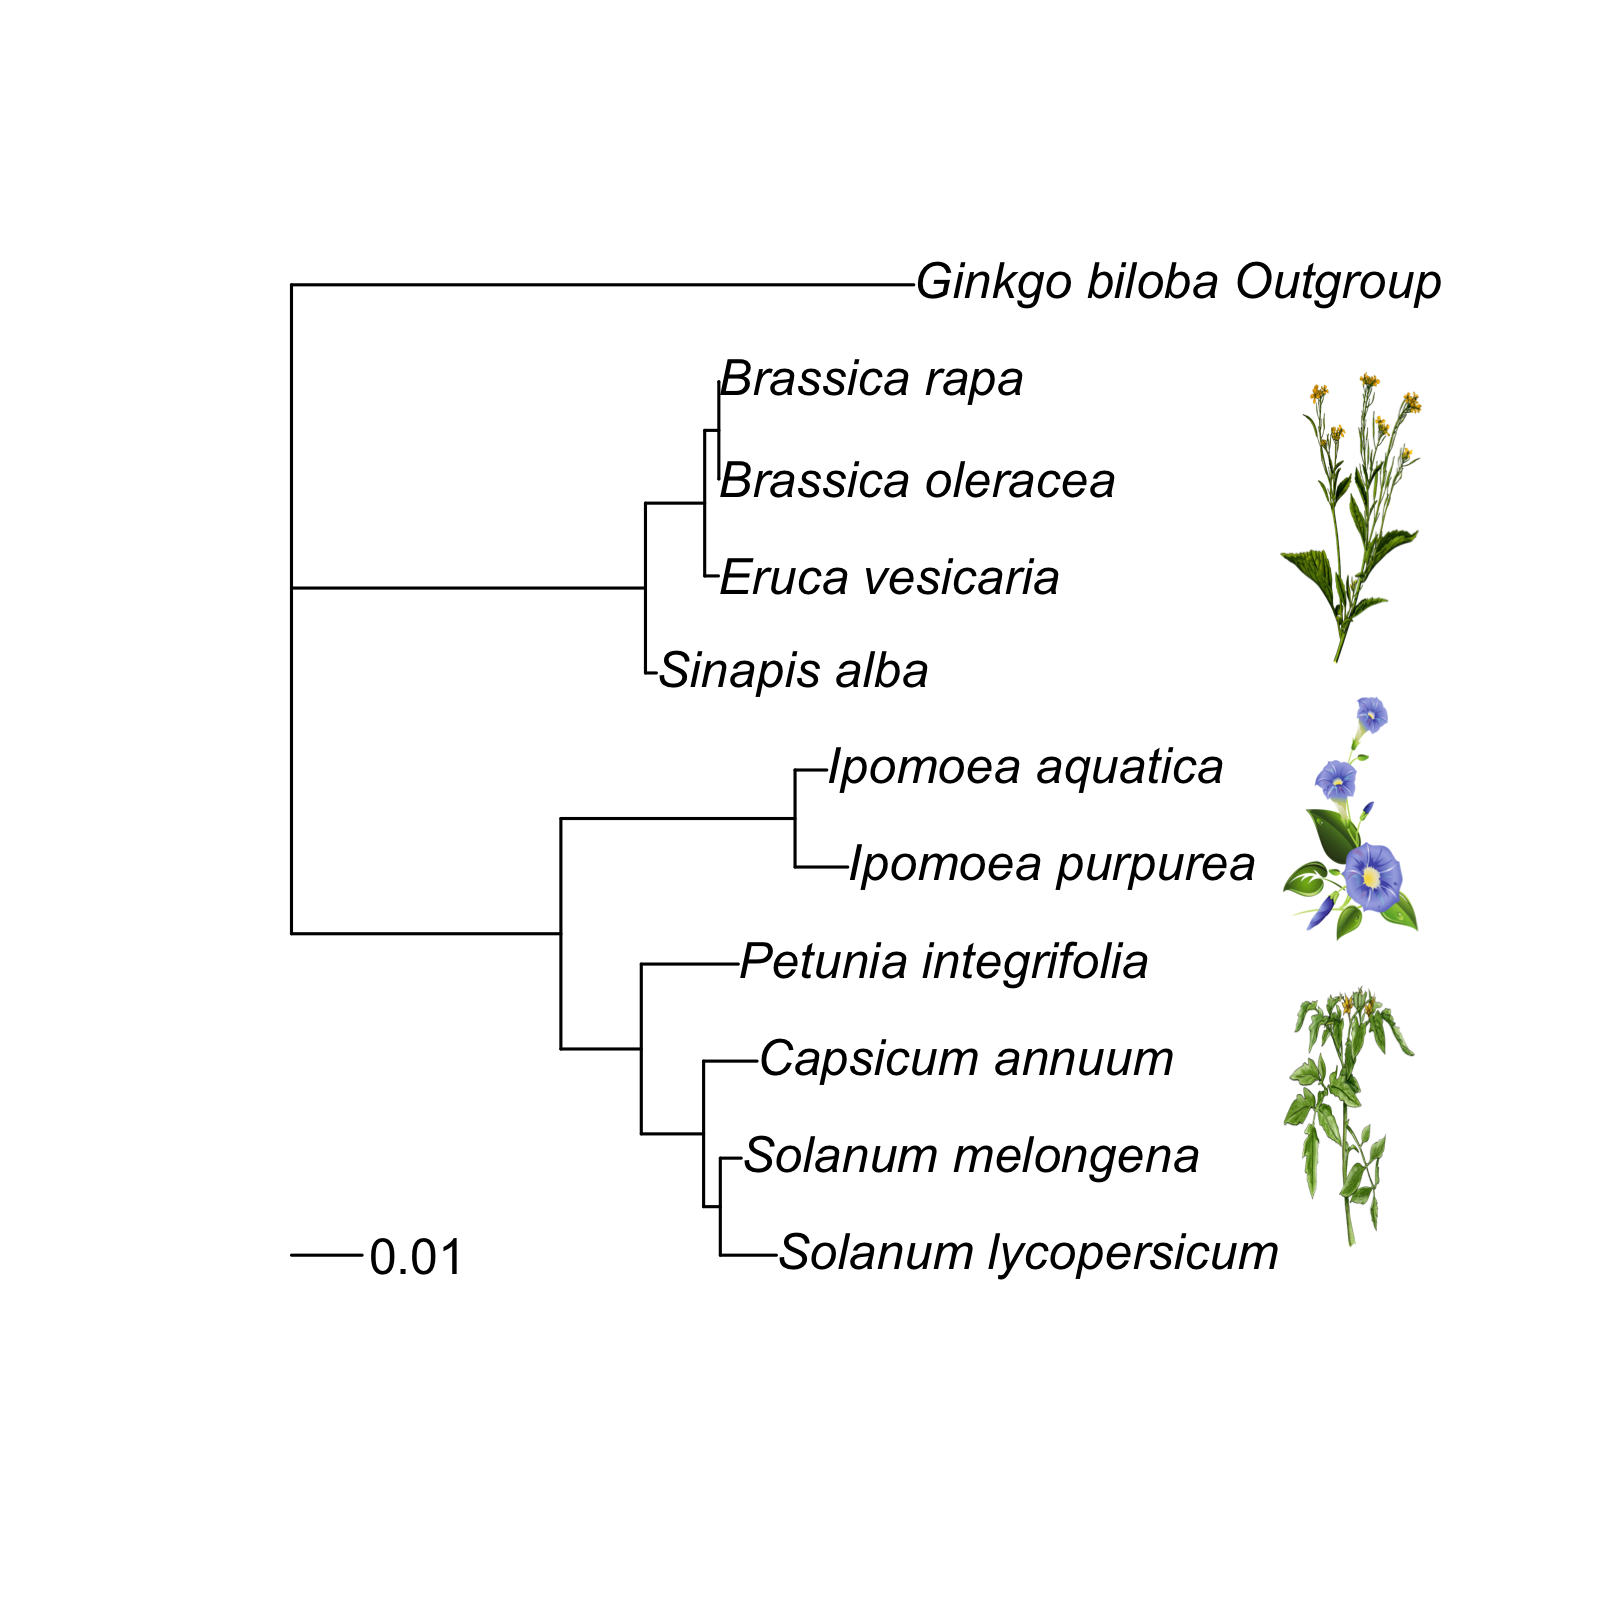
\includegraphics[width=1\linewidth]{images/phylo_image} \textbf{Figure
1} \newpage

\begin{center}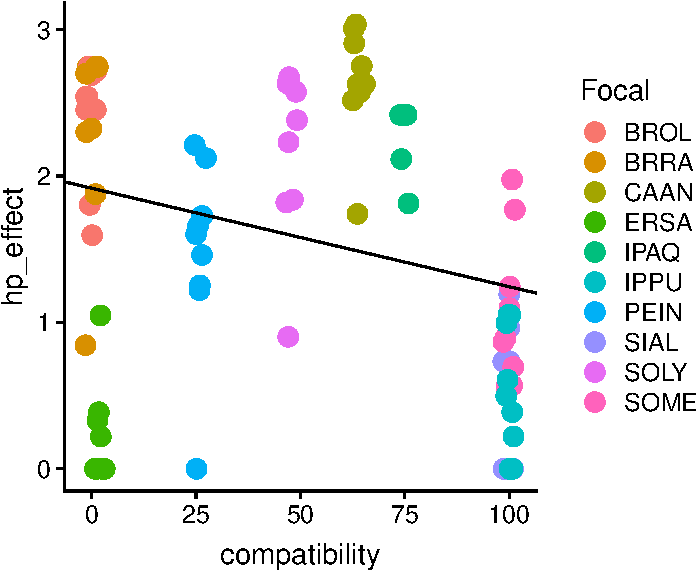
\includegraphics{output/figures/unnamed-chunk-4-1} \end{center}

\textbf{Figure 2}

\newpage

\begin{center}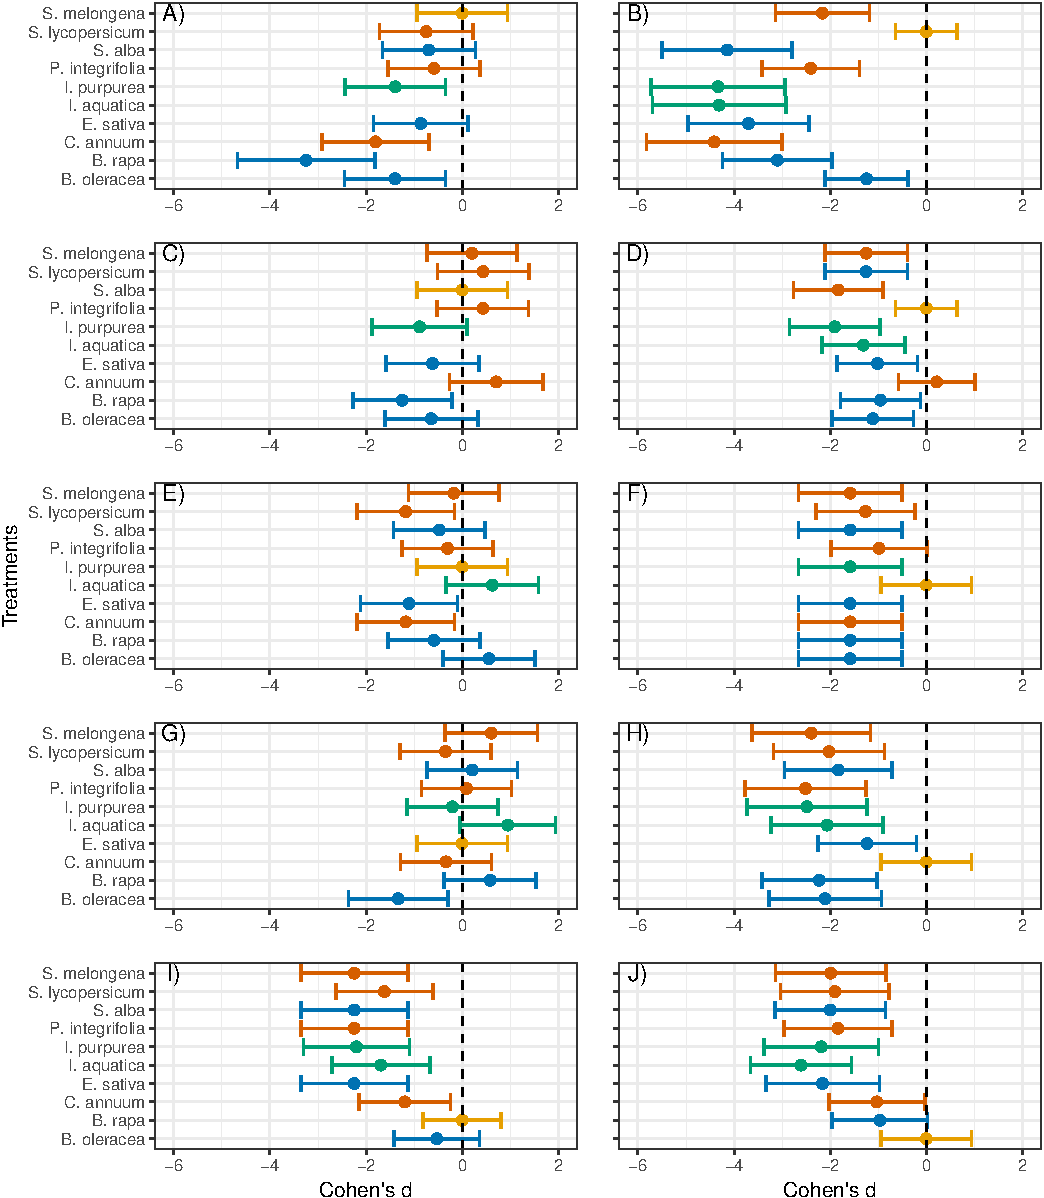
\includegraphics{output/figures/unnamed-chunk-5-1} \end{center}

\textbf{Figure 3}

\newpage

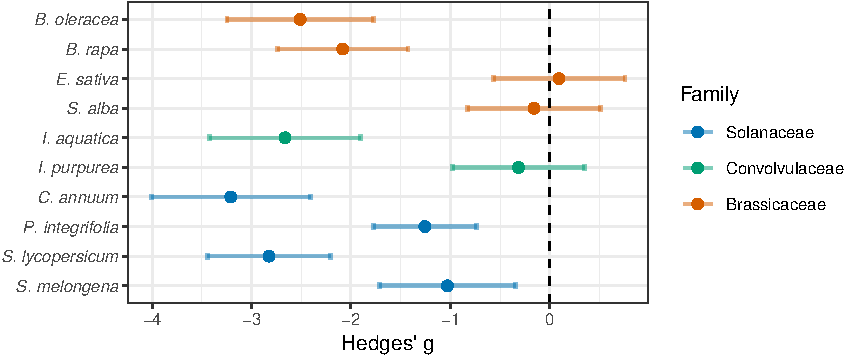
\includegraphics{output/figures/unnamed-chunk-6-1.pdf} \textbf{Figure 4}

\newpage

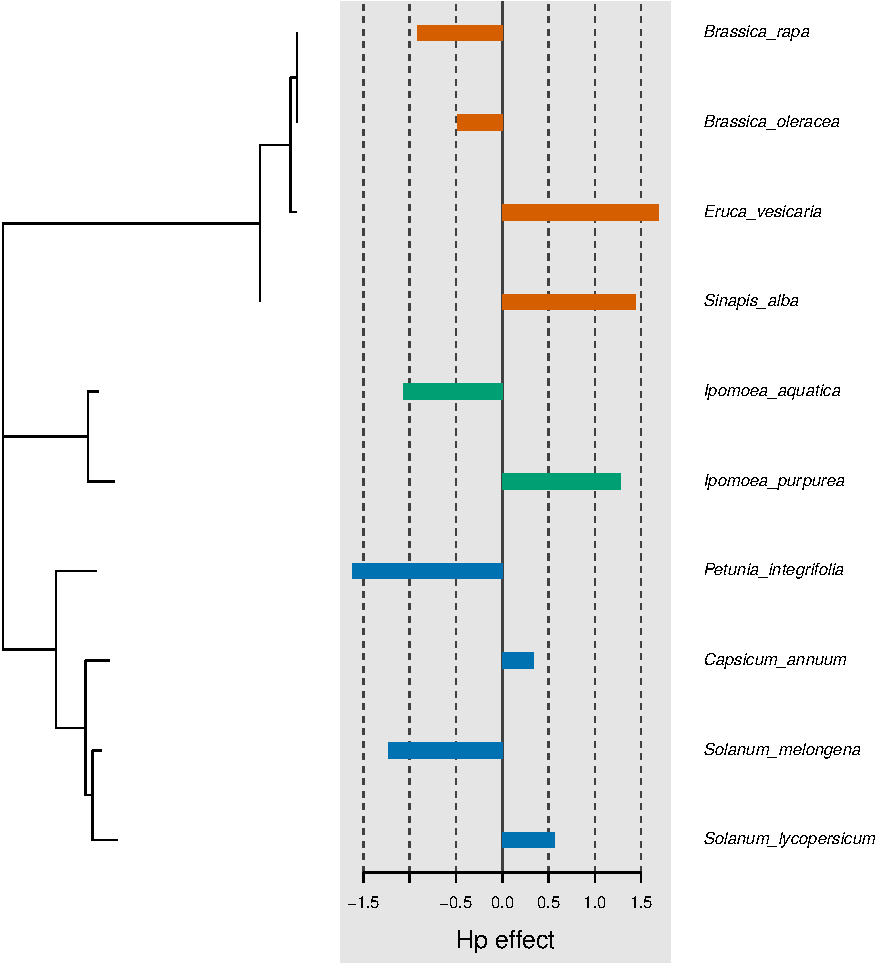
\includegraphics{output/figures/unnamed-chunk-7-1.pdf} \textbf{Figure 5}

\newpage

\begin{center}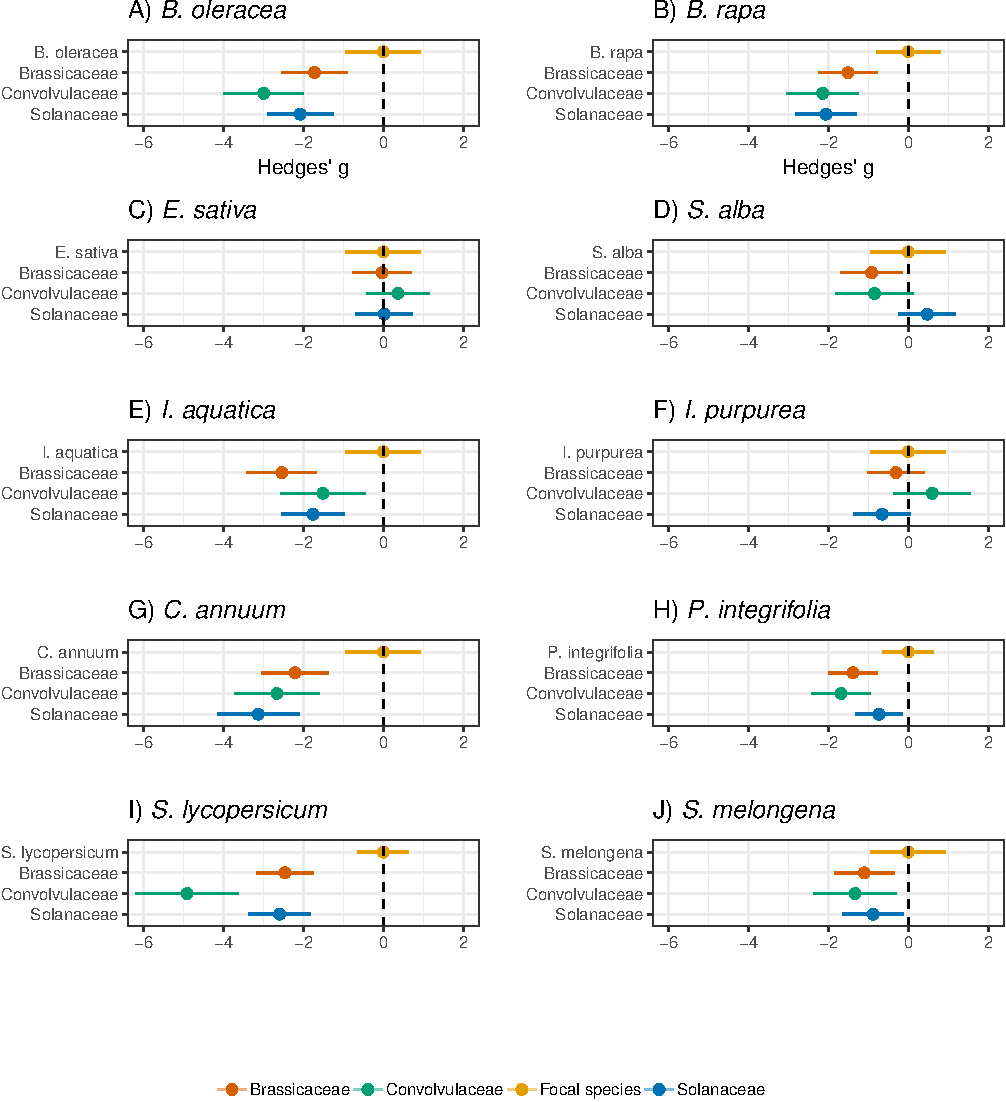
\includegraphics{output/figures/unnamed-chunk-8-1} \end{center}

\textbf{Figure 6}

\newpage

\begin{center}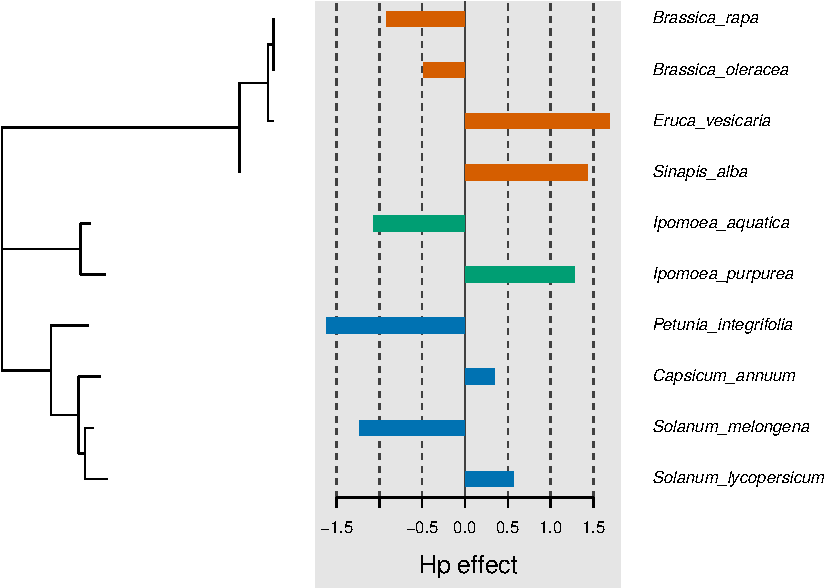
\includegraphics{output/figures/unnamed-chunk-9-1} \end{center}

\textbf{Figure 8}

\newpage

\begin{center}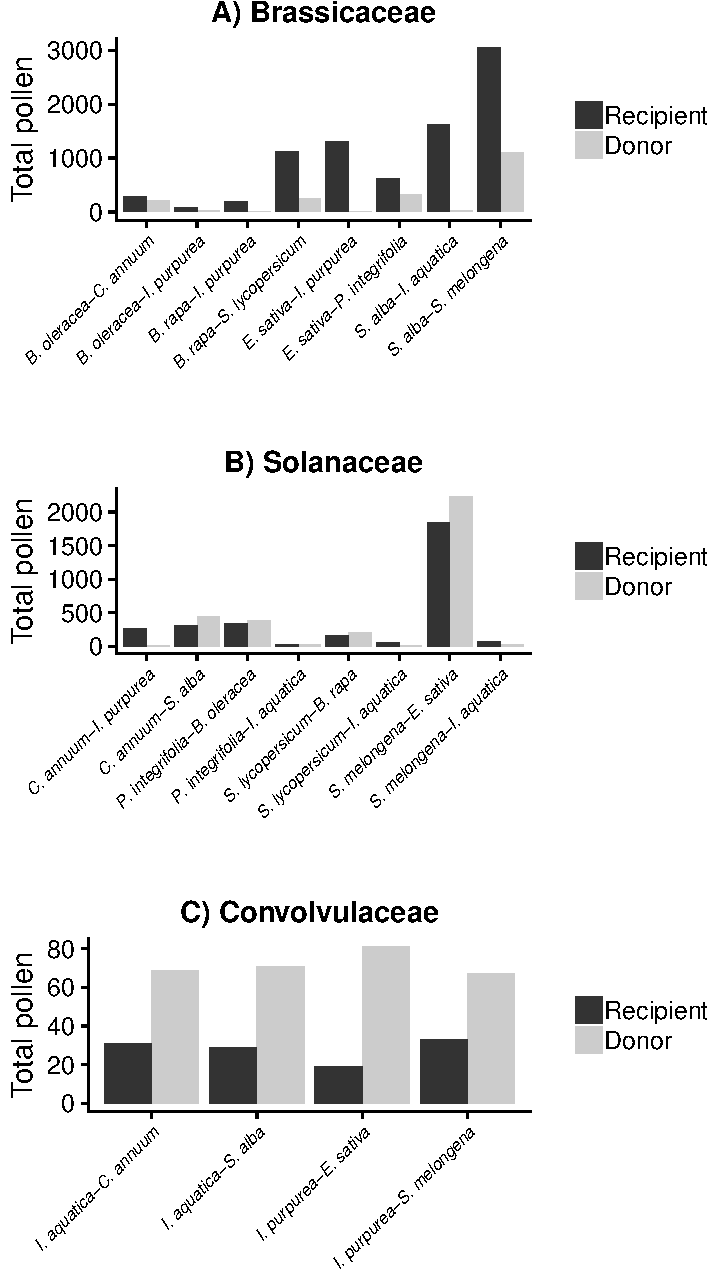
\includegraphics{output/figures/unnamed-chunk-10-1} \end{center}

\textbf{Figure 9}

\newpage

\section{List of tables}\label{list-of-tables}

\textbf{Table 1} Species list with family and genus.

\textbf{Table 2} Results of hand corss-pollination, hand
self-pollination, natural selfing (unpollinated bagged flowers) and
apomixis. The values are the average seed production per treatment
(N=10) divided by the average number of ovules per species.

\textbf{Table 3} Seed production for the treatments that produced seeds
with 100\% foreign pollen.

\section{List of figures}\label{list-of-figures}

\textbf{Figure 1} Phylogenetic tree of the species used in the
experiment from three different families from top to bottom:
Brassicaceae, Convolvulaceae and Solanaceae.

\textbf{Figure 2} Barplot of the different tests of the reproductive
biology of the species. The y axis is the percentage of ovules converted
to seed. The different treatments are, hand cross-pollination, hand
self-pollination, natural selfing and apomixis (N=10 for all of them).

\textbf{Figure 3} The impact of foreign pollen on recipient plant
species. Effect sizes (with 95\% confidence intervals) of 9 different
donor species of heterospecific pollen upon all recipients.

\textbf{Figure 4} The response of heterospecific pollen upon 10
recipient plant species. Each panel represents one recipient plant
species crossed with 50\% mixes of the other 9 species.

\textbf{Figure 5} The impact of foreign pollen on recipient plant
species. Effect sizes (with 95\% confidence intervals) of the species
grouped per family upon all recipients.

\textbf{Figure 6} Phylogenetic signal of hterospecific pollen effect
(hedges' g)

\textbf{Figure 7} (comment) Simple Pearson correlation in order to show
a possible path to follow in the article showing that style length and
stigma size could explain the effect in Solanaceae species.

\textbf{Figure 8} Pollen ratio counts on stigma after hand pollination
with 50-50\% mix. The panel is divided by family: A) Brassicaceae, B)
Convolvulaceae and C) Solanaceae. The pollen recipient species is
coloured in black and the donor species in grey.

\textbf{Figure 9} Total pollen counts on stigma after hand pollination
with 50-50\% mix. The panel is divided by family: A) Brassicaceae, B)
Convolvulaceae and C) Solanaceae. The pollen recipient species is
coloured in black and the donor species in grey.


\end{document}
